\documentclass[11pt]{article}
\title{Geant4 Benchmark Analysis: Al cube and He cylindrical chamber}
\author{Shaun Marshall}
\date{\today}
\usepackage{abstract}
\usepackage{multicol}
\usepackage{anysize}
\usepackage{graphicx}
\usepackage{float}

% Figures within a column...
\makeatletter
\newenvironment{tablehere}
{\def\@captype{table}}
{}
\newenvironment{figurehere}
{\def\@captype{figure}}
{}
\makeatother

\marginsize{1 in}{1 in}{1 in}{1 in}
\begin{document}
\maketitle

\begin{abstract}\emph{
This experiment analyzes a setup of interest, firing collimated protons at varying decades of energy at an aluminum box 50 cm away of side 5, 10, and 25 cm, 50 cm in front of a cylindrical container of helium.  The analytical tasks with which to assess and characterize the scenario include an energy deposition map, charge displacemnent map, and particle creation probabilities tables.  Results are comparable to empirical studies of proton dosimetry and demonstrate sensitivity of Geant4.
}\end{abstract}

\begin{multicols}{2}

\section{Introduction}

\section{Procedure}

Collimated protons were fired at the Al block from 50 cm away, which lie in front of a cylindrical He gas chamber centered in line with the block vertically, perpendicular to the cylinder's long axis; the solid geometry lie in a vacuum (fig~\ref{fig:schematic}).  This geometry was adjusted and retested for the 5, 10 and 25 cm side lengths  of the Al.  Energy deposition and net charge transfer by millimeter is recorded and normalized per primary proton.  Proton and neutron production combitions are found in time with gamma ray creation.  The resulting data were plotted with Gnuplot.

\begin{figurehere}
\centering
\resizebox{\columnwidth}{!}{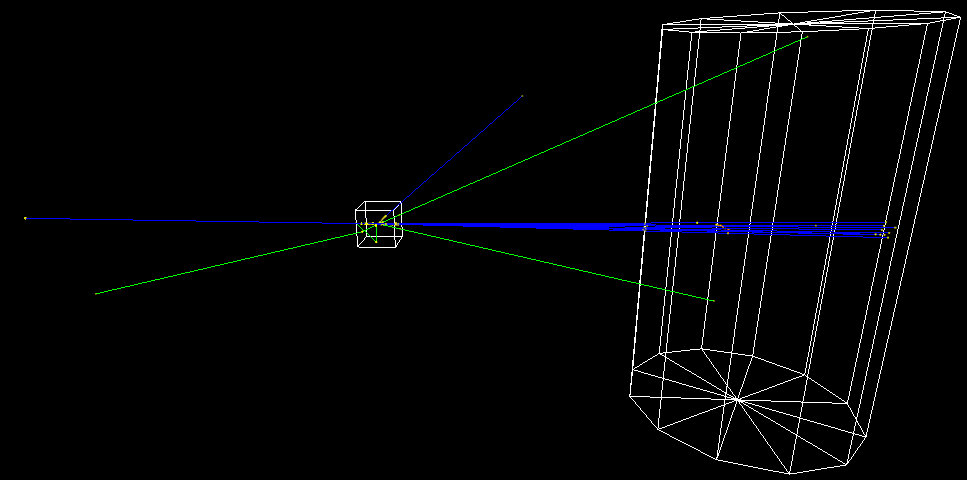
\includegraphics{../testrun.png}}
\caption{\label{fig:schematic}\small \emph{Schematic of constructed detector geometry with sample event}}
\end{figurehere}

\section{Discussion}

\section{Conclusion}

\end{multicols}
\end{document}
